\section{Discussion}

\begin{figure}[ht]
  \centering{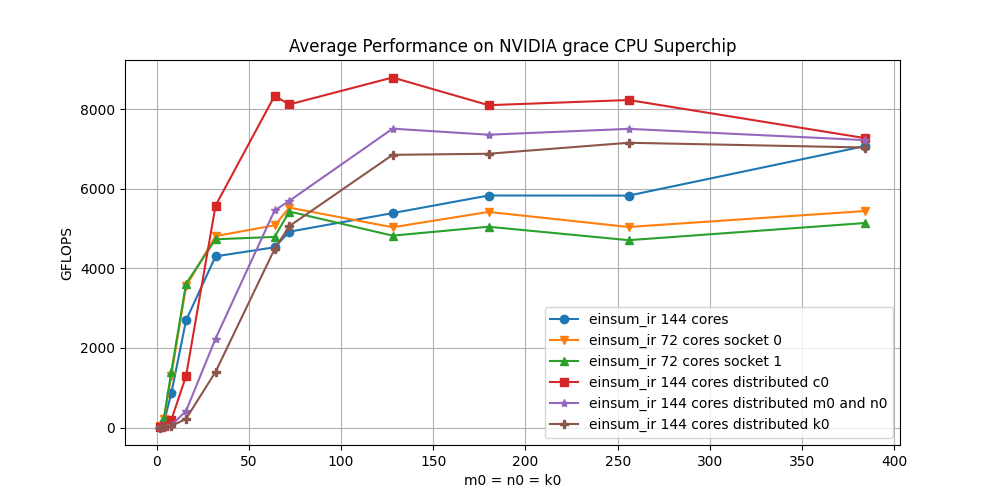
\includegraphics[width=0.95\textwidth]{gflops_grace.png}
  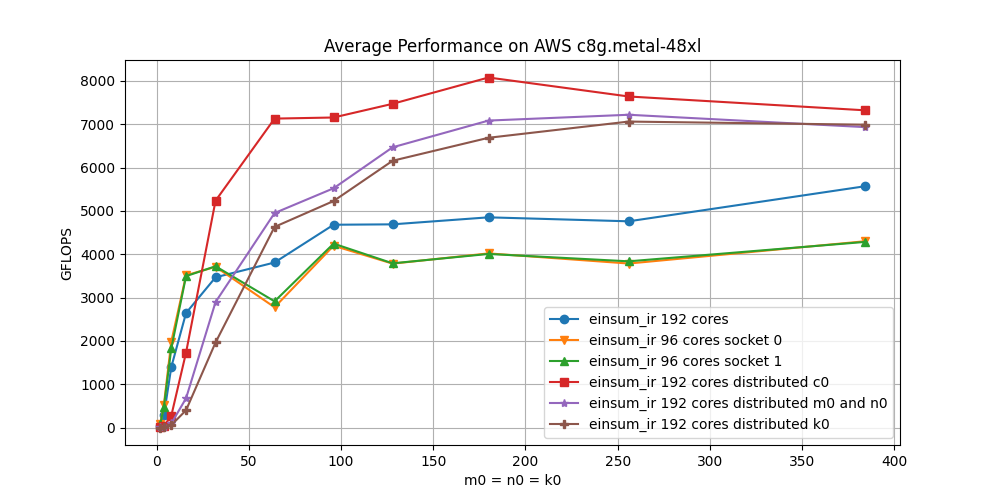
\includegraphics[width=0.95\textwidth]{gflops_g8c.png}
  }
  \caption{
    Performance of \texttt{einsum\_ir} on a dual socket NVIDIA Grace CPU Superchip and on a dual socket g8c.metal-48xl Graviton AWS instance.
    The contraction is $m_0c_0k_0k_1m_1, n_0c_0k_0n_0n_1 \rightarrow m_0n_0c_0n_1m_1$ with $|c_0|=2$, $|m_0|=|n_0|=|k_0|$ and $|m_1|=|n_1|=|k_1|=70\text{ on Grace and } 94\text{ on Graviton}$.
    Grace has 72 cores per NUMA domain; Graviton has 96.
    }
  \label{fig:einsum_ir_perf}
\end{figure}

\begin{figure}[ht]
  \centering{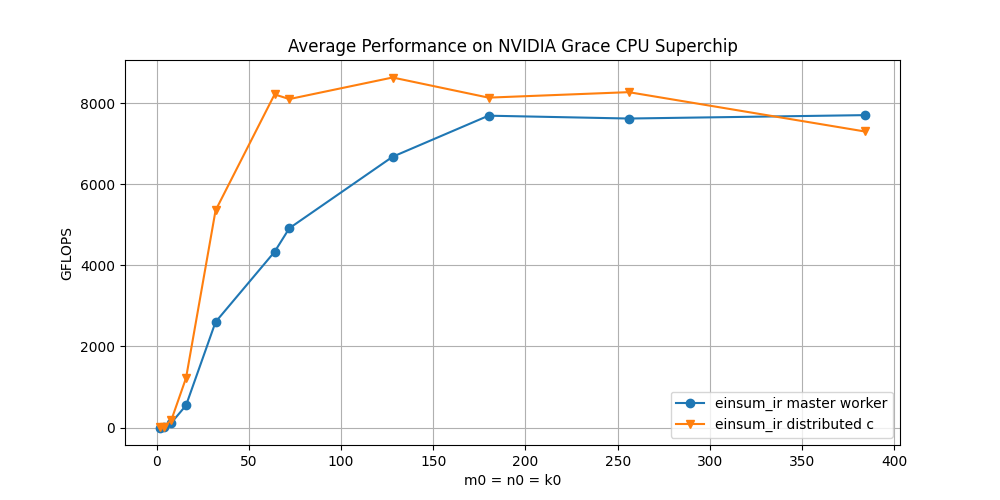
\includegraphics[width=0.95\textwidth]{gflops_grace_master_worker.png}
  }
  \caption{
    Performance of \texttt{einsum\_ir} distributed c algorithm and the master worker algorithm on a dual socket NVIDIA Grace CPU Superchip.
    The contraction is $c_0m_0k_0k_1m_1, c_0n_0k_0n_0n_1 \rightarrow c_0m_0n_0n_1m_1$ with $|c_0|=2$, $|m_0|=|n_0|=|k_0|$ and $|m_1|=|n_1|=|k_1|=70$.
    Grace has 72 cores per NUMA domain.
    }
  \label{fig:master_worker_perf}
\end{figure}

